\documentclass[a4paper, 11pt, french]{article}

\usepackage[french]{babel}
\usepackage[utf8]{inputenc}
\usepackage[T1]{fontenc}
\usepackage{csquotes}
\usepackage{amsmath,amsfonts,amssymb,mathrsfs}
\usepackage[includeheadfoot, hmargin=2cm, top=0.9cm, bottom = 1.8cm, headsep=2cm]{geometry}
\usepackage{lmodern} %pas pixelisé
\usepackage{engrec,titlesec,lipsum,xcolor}
\usepackage{fancybox}
\usepackage[skins, most]{tcolorbox}
\usepackage[bookmarks={true},bookmarksopen={true}, pdftitle={Cahier des charges}, pdfauthor={Chevalier Romain}, pdfsubject={Caméra domes}, colorlinks=true, linkcolor=black, urlcolor=blue, citecolor=red]{hyperref}
\usepackage{setspace}
\usepackage{stmaryrd}
\usepackage{multicol} 
\usepackage{enumitem}
\usepackage{array,multirow,makecell}
\usepackage{titlesec}
\usepackage{multirow}
\usepackage{hyperref}
\usepackage{listings}
\usepackage{graphicx}
\usepackage{caption}
\usepackage{subcaption}
\usepackage{float}
\usepackage{fancyhdr}
\usepackage[bottom]{footmisc}
\usepackage{footnote}
\usepackage[page,header]{appendix}
\usepackage{titletoc}
\makesavenoteenv{tabular}
\makesavenoteenv{table}

\graphicspath{{Figures/}{Photos/}}

\usepackage{tikz}
\usepackage{pgfplots}
\usetikzlibrary{decorations.pathmorphing, shapes, automata,positioning}



%-----------------------------------------------------------------------------------

\pagestyle{fancy}
\renewcommand{\headrulewidth}{1pt}
\fancyhead[C]{\leftmark} 
%\fancyhead[R]{\includegraphics[scale=0.13]{logoAdeoService.jpg}}
\fancyhead[R]{
\includegraphics[scale=0.1]{Logo_CENTRALE_C.png}}
\newcolumntype{M}{>{\centering\arraybackslash}m{1.75cm}}
\setlength{\headheight}{30.5pt}

%-----------------------------------------------------------------------------------

\frenchbsetup{StandardLists=true}
%\setlength{\parskip}{1em}
\AddThinSpaceBeforeFootnotes
\FrenchFootnotes

%---------------------------------------------------------------

%-----------------------------------------------------------------------------------

\definecolor{vert}{rgb}{0,0.69,0.31}
\definecolor{bleue}{rgb}{0,0.31,0.69} 
\definecolor{violet}{rgb}{0.38,0.18,055} % 97, 45, 140     244, 208, 63
\definecolor{jaune}{rgb}{0.96, 0.85, 0.23}

\definecolor{darkWhite}{rgb}{0.94,0.94,0.94}
\definecolor{vert}{rgb}{0,0.69,0.31}
\definecolor{rose}{rgb}{1,0.08,0.58}% rgb(255,20,147)
\definecolor{rouge}{rgb}{0.78,0.12,0.08}
\definecolor{gris}{rgb}{0.4,0.4,0.4}
\definecolor{marron}{rgb}{0.4,0.2,0}
\definecolor{darkWhite}{rgb}{0.94,0.94,0.94}

%-----------------------------------------------------------------------------------

\title{%
        \Huge Suivi d'un grimpeur par caméra dome \\
        \LARGE Rapport de PDI}

\author{\LARGE CHEVALIER Romain}
\date{\today}

\newcommand{\hsp}{\hspace{20pt}}
\newcommand{\HRule}{\rule{\linewidth}{0.5mm}}

%-----------------------------------------------------------------------------------

\newcounter{obj}
\setcounter{obj}{1}


%-----------------------------------------------------------------------------------


\begin{document}
\pagenumbering{roman}
\begin{titlepage}

    \begin{titlepage}
        \begin{center}
      
          % Upper part of the page. The '~' is needed because \\
          % only works if a paragraph has started.
      
          \textsc{\LARGE École Centrale De Lille}\\[2cm]
      
          \textsc{\huge Projet d'intégration}\\[2cm]
      
          % Title
          \HRule \\[0.4cm]
          { \Huge \bfseries Suivi d'un grimpeur par caméra dome\\[0.4cm] }
      
          \HRule \\[2cm]

          \textsc{\Large Rapport de PDI \\} {\large\today}\\[1.5cm]
          
          \vfill
          % A cahnger pour les caméras installées 
          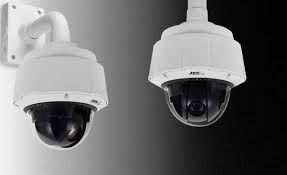
\includegraphics[width=.8\textwidth]{Figures/cameraQ6304.jpg}
          \vfill

          % Author and supervisor
          \begin{minipage}{0.4\textwidth}
            \begin{flushleft} \large
              CHEVALIER Romain\\
            \end{flushleft}
          \end{minipage}
          \begin{minipage}{0.4\textwidth}
            \begin{flushright} \large
              \emph{Tuteur :}  BOURDEAUD'HUY T. \\
            \end{flushright}
          \end{minipage}
      
          \vspace{1cm}
         
        \end{center}
      \end{titlepage}
    
    \normalsize
   
\end{titlepage}

%-----------------------------------------------------------------------------------

\setcounter{secnumdepth}{3}
\setcounter{tocdepth}{3}
\startcontents[sections]

%-----------------------------------------------------------------------------------
\tableofcontents
%\printcontents[sections]{l}{1}{\setcounter{tocdepth}{3}}
%\printcontents[sub]{l}{1}{\setcounter{tocdepth}{2}}
\pagenumbering{arabic}
\newpage

%-------------------------------------------------------------

\section{Contexte}
Afin d'améliorer les services offerts aux utilisateurs de la salle d’escalade \textit{Sac à Pof} situé à  Mons-en-Barœul (59), on envisage de mettre en place un système de suivi automatisé des grimpeurs à l'aide de caméras IP dômes motorisées. Ces caméras permettront de suivre les mouvements des grimpeurs sur les différentes voies en ajustant automatiquement le cadrage et le zoom en fonction de leur position. Le services sera accessible via une application web hébergée sur un serveur local. Cette solution vise à offrir un support d'analyse post-session, afin de permettre aux grimpeur de comprendre leurs forces et faiblesses pour s'améliorer.

Afin de réalisé ce projet, nous sommes en possession de deux caméras IP dômes motorisées de la marque \textit{AXIS} modèle \textit{Q6304-E\footnote{Voir \href{https://www.axis.com/dam/public/11/e4/20/cam\%C3\%A9ra-r\%C3\%A9seau-\%C3\%A0-d\%C3\%B4me-ptz-axis-q6034-e-fr-FR-201515.pdf}{fiche technique} pour plus d'informations}}, d'un routeur, d'une tablette Android et d'un raspberry pi 4.

\subsection{Objectifs}
Les objectifs de ce projet sont multiples et sont résumés dans la liste suivante :
\begin{itemize}
  \item Prendre en main les caméras IP dômes motorisées et les intégrer dans un réseau local.
  \item Développer une interface web permettant de piloter les caméras, l'enregistrement de video et leur visualisation.
  \item Avoir un retour visuel de la caméra en temps réel sur l'interface web.
  \item Développer une méthode de communication entre l'application web et les programmes de contrôle des caméras.
  \item Développer un algorithme de suivi de grimpeur en temps réel.
  \item Développer une méthode permettant d'enregister sur un stockage une vidéo.
  \item Avoir une application modulable permettant de modifier les caméra et les paramètres de détection.
\end{itemize}

\section{Architecture du système}
\subsection{Architecture matérielle}
Le système est composé de plusieurs éléments qui interagissent entre eux, la figure \ref{fig:architecture} montre l'architecture du système. Le système repose sur un \textbf{Raspberry Pi 4}, qui joue un rôle central en assurant la communication entre les différentes composantes. Il est connecté au réseau local via un \textbf{routeur}, qui agit comme un serveur DHCP, attribuant dynamiquement les adresses IP aux appareils du système.

Les \textbf{caméras Dome IP} sont accessibles via HTTP et envoient leur flux vidéo vers le Raspberry Pi lorsqu’elles sont activées. Ces caméras disposent de positions prédéfinies correspondant aux différentes voies d’escalade, mais peuvent également être orientées dynamiquement par l’utilisateur via la \textbf{tablette} fournie ou tout autre appareil connecté au réseau local.

Le Raspberry Pi exécute un serveur d’application web,ce serveur permet :
\begin{itemize}
    \item de piloter les caméras (changement de position, orientation manuelle),
    \item de gérer les enregistrements vidéo,
    \item de stocker dans une base de données les vidéos enregistrées ainsi que les positions des caméras définies par l’utilisateur.
\end{itemize}

L’enregistrement des vidéos est déclenché manuellement depuis l’interface de la tablette et les fichiers sont conservés jusqu’à suppression par l’utilisateur.

L’architecture ainsi mise en place assure une gestion centralisée et accessible du système, tout en permettant un contrôle précis et flexible des caméras et des enregistrements.


\begin{figure}[!ht]
  \centering
  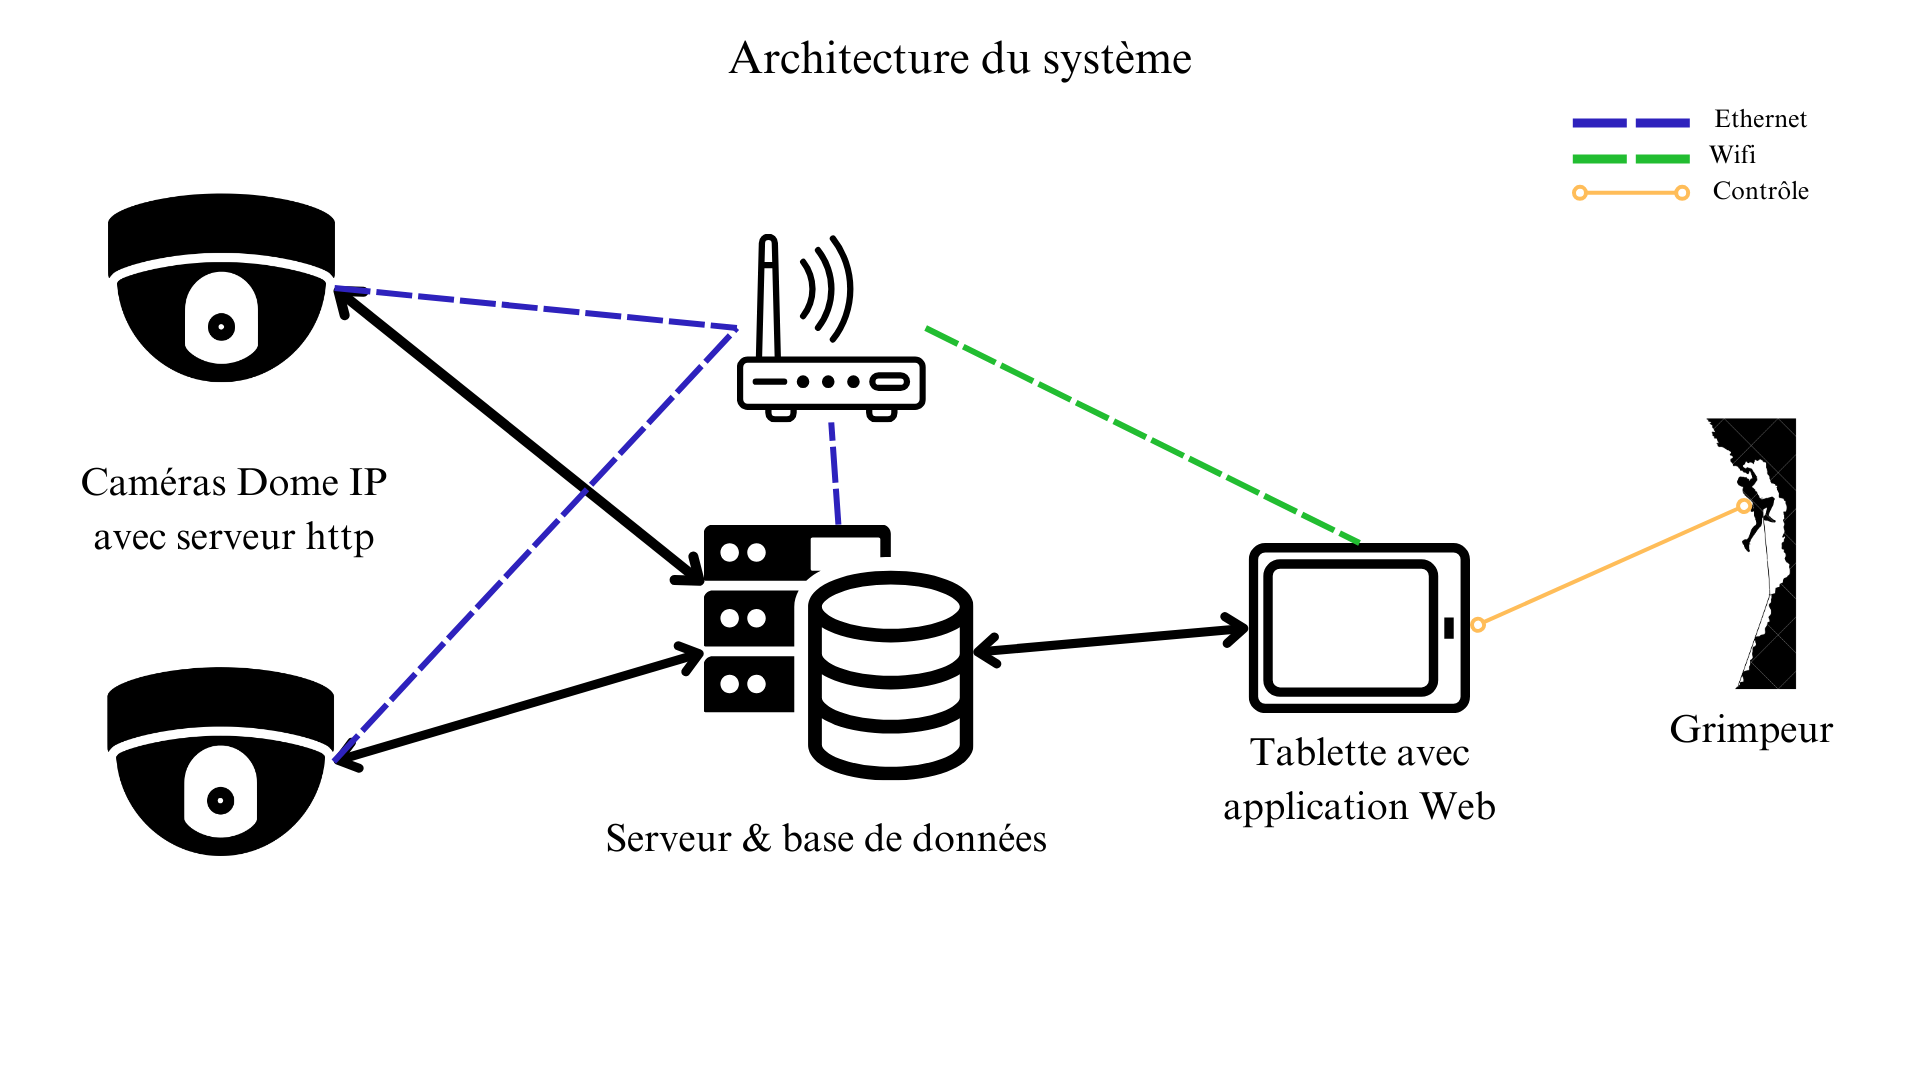
\includegraphics[width=\textwidth]{architectureMaterielle.png}
  \caption{Architecture du système}
  \label{fig:architecture}
\end{figure}

\subsection{Architecture logicielle}
L'architecture logicielle du système est représentée sur la figure \ref{fig:architectureLogicielle}. Le raspberry Pi divise ses tâches en deux parties distinctes : le serveur web et la partie gestion de l'application développée. En fonction des actions effectuées sur la page web, le serveur apache exécuté deux scripts \texttt{cgi} différents, le premier script, nommé \textbf{video.cgi} codé en \texttt{c++}, démarre au chargement de la page permet d'afficher le flux vidéo de la caméra sur la page web en lisant les images brutes dans la mémoire partagée et en les encodant en \texttt{JPEG}. Le second (\textbf{action.cgi} développé en \texttt{c}) permet de transmettre les ordres de déplacement de la caméra ou lancer un enregistrement vidéo via l'écriture de cet ordre dans un segment de mémoire partagé puis de réveillé le programme principal en lui envoyant un signal. 


De l'autre côté, le programme principal (\textbf{main} programmé en \texttt{c}) est en charge de la gestion des caméras, de la détection de mouvement et de l'enregistrement des vidéos. Au démarrage, il crée un processus fils (\textbf{écriture mémoire})qui est en charge de récupérer le flux vidéo du serveur HTTP de la caméra et de le stocker en image brute dans une mémoire partagée. Le programme principal est ensuite en attente d'un signal pour effectuer une action, comme le déplacement de la caméra, l'enregistrement de position ou encore le lancement d'un enregistrement qui va crée un processus fils (\textbf{enregistrement vidéo}) qui encode le flux video en \texttt{MP4} afin de le stocker sur le disque dur et lance la détection du grimpeur pour suivre ces mouvements à l'aide d'un second fils (\textbf{détection}). Ces deux processus récupèrent les images en lisant la mémoire partagée et les traitent pour effectuer leur tâche. Enfin, le programme de détection peut directement agir sur la position de la caméra en lui envoyant une requête HTTP.


\begin{figure}[!ht]
  \centering
  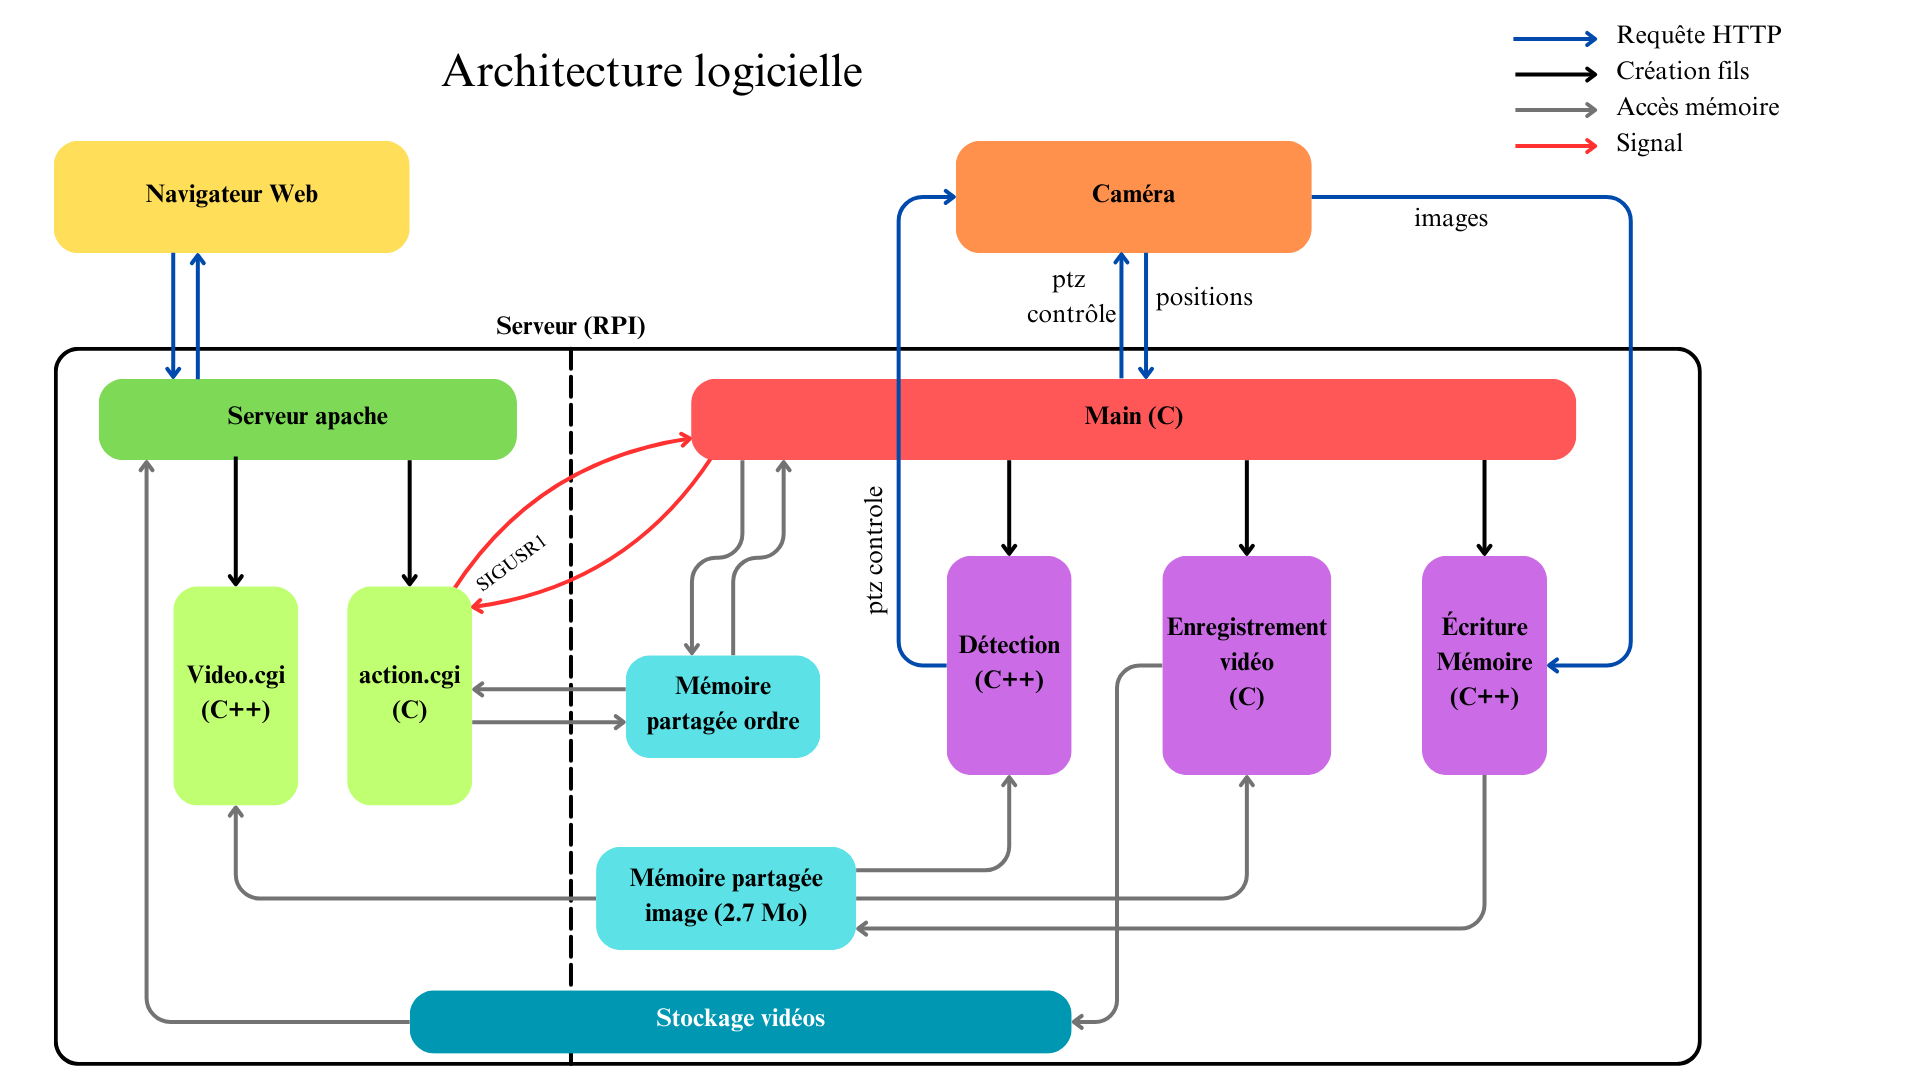
\includegraphics[width=\textwidth]{architectureLogicielle.png}
  \caption{Architecture logicielle}
  \label{fig:architectureLogicielle}
\end{figure}


%-----------------------------------------------------------

\section{Développement de l'application}
Dans cette partie, nous allons détailler les différentes étapes de développement de l'application pour chaque brique du système présent dans l'architecture logicielle en figure \ref{fig:architectureLogicielle}.

%-----------------------------------------------------------
\subsection{Application système}

Le programme principal est le cœur du système, il est en charge de faire la liaison avec entre le serveur web et les différents processus, de piloter la caméra et de gérer les positions remarquables de la caméra. 

\subsubsection{Programme principal}

Le fichier \texttt{main.c} constitue le cœur du système de gestion des caméras et de la communication inter-processus. Il est responsable de l'initialisation des caméras, de la gestion des enregistrements vidéo, de la détection des mouvements, et de l'interaction avec l'interface CGI via des segments de mémoire partagée et des sémaphores.

\paragraph{Initialisation du programme}
Lors de son démarrage, le programme effectue plusieurs étapes d'initialisation :
\begin{itemize}
    \item \textbf{Gestionnaire de fin d'exécution} : La fonction \texttt{atexit(bye)} garantit que toutes les ressources (mémoire partagée, sémaphores, processus enfants) sont correctement libérées à la fin du programme.
    \item \textbf{Initialisation des sémaphores} : La fonction \texttt{initSemaphores()} crée ou ouvre des sémaphores nommés pour synchroniser les processus et gérer l'accès à la mémoire partagée, voir le paragraphe~\ref{par:semaphores} pour leur fonctionnement.
    \item \textbf{Initialisation de la mémoire partagée} : La fonction \texttt{initSegmentMemoire()} configure deux segments de mémoire partagée : un pour les ordres envoyés par l'interface CGI et un autre pour stocker les images brutes capturées par les caméras.
    \item \textbf{Initialisation des caméras} : La fonction \texttt{initCamera()} charge les paramètres des caméras depuis un fichier JSON et configure les caméras actives.
\end{itemize}

\paragraph{Gestion des signaux}
Le programme installe un gestionnaire de signaux (\texttt{signalHandler}) pour répondre aux événements suivants :
\begin{itemize}
    \item \textbf{SIGINT} : Interruption manuelle (Ctrl+C) pour arrêter le programme proprement.
    \item \textbf{SIGCHLD} : Gestion des processus enfants terminés pour éviter les processus zombies.
    \item \textbf{SIGUSR1} : Signal utilisé pour indiquer qu'un nouvel ordre a été reçu via la mémoire partagée.
\end{itemize}

\paragraph{Boucle principale}
Le programme entre dans une boucle infinie en appelant \texttt{pause()}, ce qui le met en attente d'un signal. Lorsqu'un signal est reçu, le gestionnaire de signaux (\texttt{signalHandler}) est exécuté pour traiter l'événement.

\paragraph{Gestion des ordres}
Lorsqu'un signal \texttt{SIGUSR1} est reçu, la fonction \texttt{gestionOrdres()} est appelée pour lire et exécuter les ordres envoyés par l'interface CGI. Les types d'ordres gérés incluent :
\begin{itemize}
    \item \textbf{Déplacement de la caméra} : Commandes de mouvement (\texttt{move}) ou de zoom (\texttt{zoom}).
    \item \textbf{Enregistrement vidéo} : Commandes d'enregistrement (\texttt{reco}) pour démarrer ou arrêter un processus de capture vidéo.
    \item \textbf{Détection de mouvement} : Commandes de détection (\texttt{detc}) pour analyser les images et suivre les mouvements.
    \item \textbf{Gestion des positions prédéfinies} : Commandes (\texttt{rout}) pour ajouter, supprimer ou afficher des positions prédéfinies.
    \item \textbf{Changement de caméra active} : Commandes (\texttt{cam}) pour basculer entre les caméras configurées.
\end{itemize}

\paragraph{Gestion des processus enfants}
Le programme utilise des processus enfants pour effectuer des tâches spécifiques :
\begin{itemize}
    \item \textbf{Processus d'écriture mémoire} : Capture le flux vidéo brut des caméras et le stocke dans la mémoire partagée.
    \item \textbf{Processus de détection} : Analyse les images pour détecter les mouvements.
    \item \textbf{Processus d'enregistrement vidéo} : Encode les images en vidéo MP4 et les stocke sur le disque.
\end{itemize}

\paragraph{Libération des ressources}
Lorsque le programme se termine, la fonction \texttt{bye()} est appelée pour libérer toutes les ressources :
\begin{itemize}
    \item Les processus enfants encore actifs sont arrêtés.
    \item Les segments de mémoire partagée sont détachés et supprimés.
    \item Les sémaphores sont fermés et supprimés.
\end{itemize}

%-----------------------------------------------------------

\subsection{\'Ecriture mémoire}

Le fichier \texttt{ecritureMemoire.cpp} est un processus dédié à la capture des images vidéo depuis une source donnée (par exemple, une caméra IP) et à leur écriture dans un segment de mémoire partagée. Ce processus est essentiel pour permettre la communication inter-processus entre les différents modules du système.

\paragraph{Initialisation du programme}
Lors de son démarrage, le programme effectue plusieurs étapes d'initialisation :
\begin{itemize}
    \item \textbf{Gestionnaire de signaux} : Le programme installe un gestionnaire de signaux (\texttt{signalHandler}) pour gérer les interruptions (\texttt{SIGINT}) et les arrêts (\texttt{SIGTERM}) de manière propre.
    \item \textbf{Ouverture des sémaphores} \label{par:semaphores}: Les sémaphores nommés sont ouverts pour synchroniser l'accès à la mémoire partagée entre les processus :
    \begin{itemize}
        \item \texttt{SEM\_READERS} : Compte les lecteurs actifs.
        \item \texttt{SEM\_WRITER} : Contrôle l'accès en écriture à la mémoire partagée.
        \item \texttt{SEM\_NEW\_FRAME} : Indique qu'une nouvelle image est disponible.
        \item \texttt{SEM\_ACTIVE\_READERS} : Compte les lecteurs actifs qui attendent une nouvelle image.
    \end{itemize}
    \item \textbf{Ouverture de la mémoire partagée} : Le segment de mémoire partagée est ouvert et mappé en mémoire virtuelle pour permettre l'écriture des images capturées.
\end{itemize}

\paragraph{Capture vidéo}
Le programme utilise OpenCV pour capturer les images vidéo depuis une source spécifiée en argument :
\begin{itemize}
    \item \textbf{Initialisation de la capture vidéo} : La capture est ouverte avec \texttt{cv::VideoCapture} en utilisant l'argument passé au programme. Les propriétés de la capture sont configurées :
    \begin{itemize}
        \item Fréquence d'images (FPS) : 25 images par seconde.
        \item Résolution : 1280x720 pixels.
    \end{itemize}
    \item \textbf{Vérification de la capture} : Si la capture ne peut pas être ouverte, le programme affiche une erreur et se termine.
\end{itemize}

\paragraph{Boucle principale}
Le programme entre dans une boucle principale pour capturer les images et les écrire dans la mémoire partagée :
\begin{itemize}
    \item \textbf{Capture d'une image} : Une image est capturée à l'aide de \texttt{cap.read(frame)}. Si la capture échoue, le programme affiche une erreur et quitte la boucle.
    \item \textbf{Écriture dans la mémoire partagée} : Le sémaphore \texttt{SEM\_WRITER} est utilisé pour bloquer l'accès en écriture pendant que l'image est copiée dans la mémoire partagée. Les données de l'image sont copiées avec \texttt{std::memcpy}.
    \item \textbf{Notification des lecteurs} : Le programme utilise le sémaphore \texttt{SEM\_NEW\_FRAME} pour notifier tous les lecteurs actifs (\texttt{SEM\_ACTIVE\_READERS}) qu'une nouvelle image est disponible.
\end{itemize}

\paragraph{Libération des ressources}
Lorsque le programme se termine (par un signal ou une erreur), il libère toutes les ressources utilisées :
\begin{itemize}
    \item \textbf{Libération de la mémoire partagée} : Le segment de mémoire partagée est détaché (\texttt{munmap}) et fermé (\texttt{close}).
    \item \textbf{Fermeture des sémaphores} : Tous les sémaphores ouverts sont fermés avec \texttt{sem\_close}.
    \item \textbf{Libération de la capture vidéo} : La capture vidéo est libérée avec \texttt{cap.release}.
\end{itemize}

\paragraph{Gestion des signaux}
Le gestionnaire de signaux (\texttt{signalHandler}) permet de gérer les interruptions et les arrêts du programme :
\begin{itemize}
    \item \textbf{SIGINT} : Interrompt immédiatement le programme.
    \item \textbf{SIGTERM} : Arrête proprement le programme en mettant fin à la boucle principale.
\end{itemize}


%-----------------------------------------------------------

\subsection{Application web}
Le serveur web est composée de deux pages web voir figure~\ref{fig:pagesWeb}, la première permet de visualiser le flux vidéo de la caméra, de la piloter et de piloter l'application. La seconde permet de visualiser les vidéos enregistrées et de les télécharger, le code de ces pages est écrit en \texttt{HTML}, \texttt{CSS} et \texttt{JAVASCRIPT} peut-être consulté sur la page \href{https://github.com/Romaiiin91/suiviGrimpeur_PDI/tree/main/server/html}{GitHub}.

\begin{figure}
  \centering
  \begin{subfigure}[b]{0.45\textwidth}
    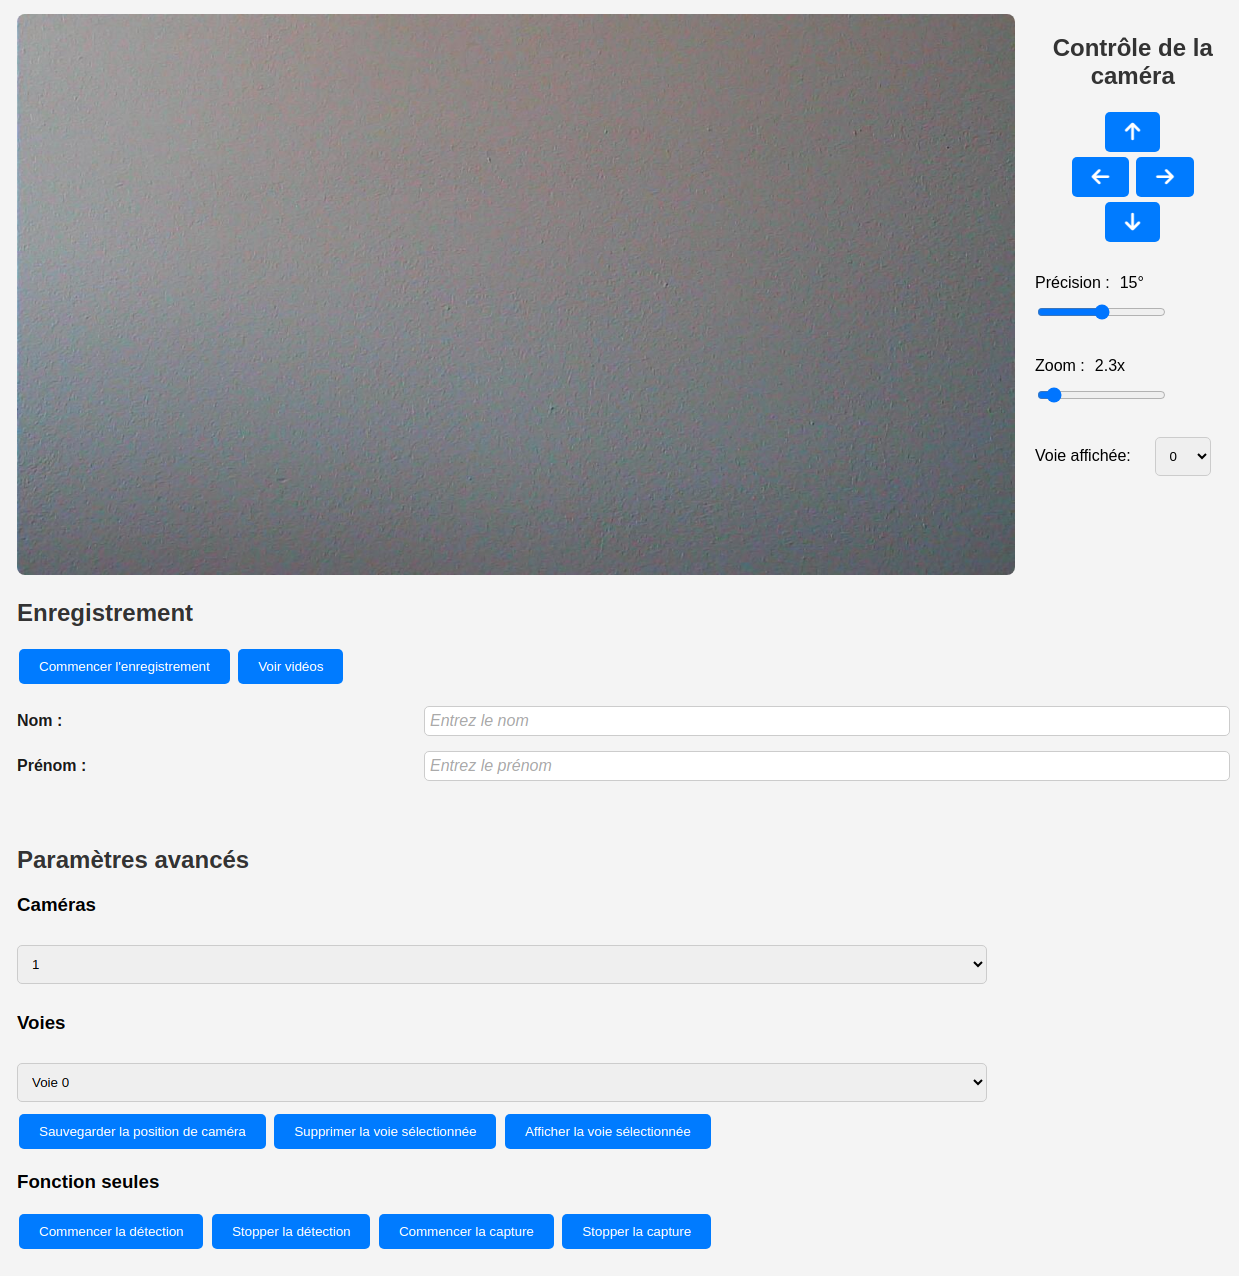
\includegraphics[width=\textwidth]{pageIndex.png}
    \caption{Index de l'application}
    \label{fig:pageIndex}
  \end{subfigure}
  \begin{subfigure}[b]{0.45\textwidth}
    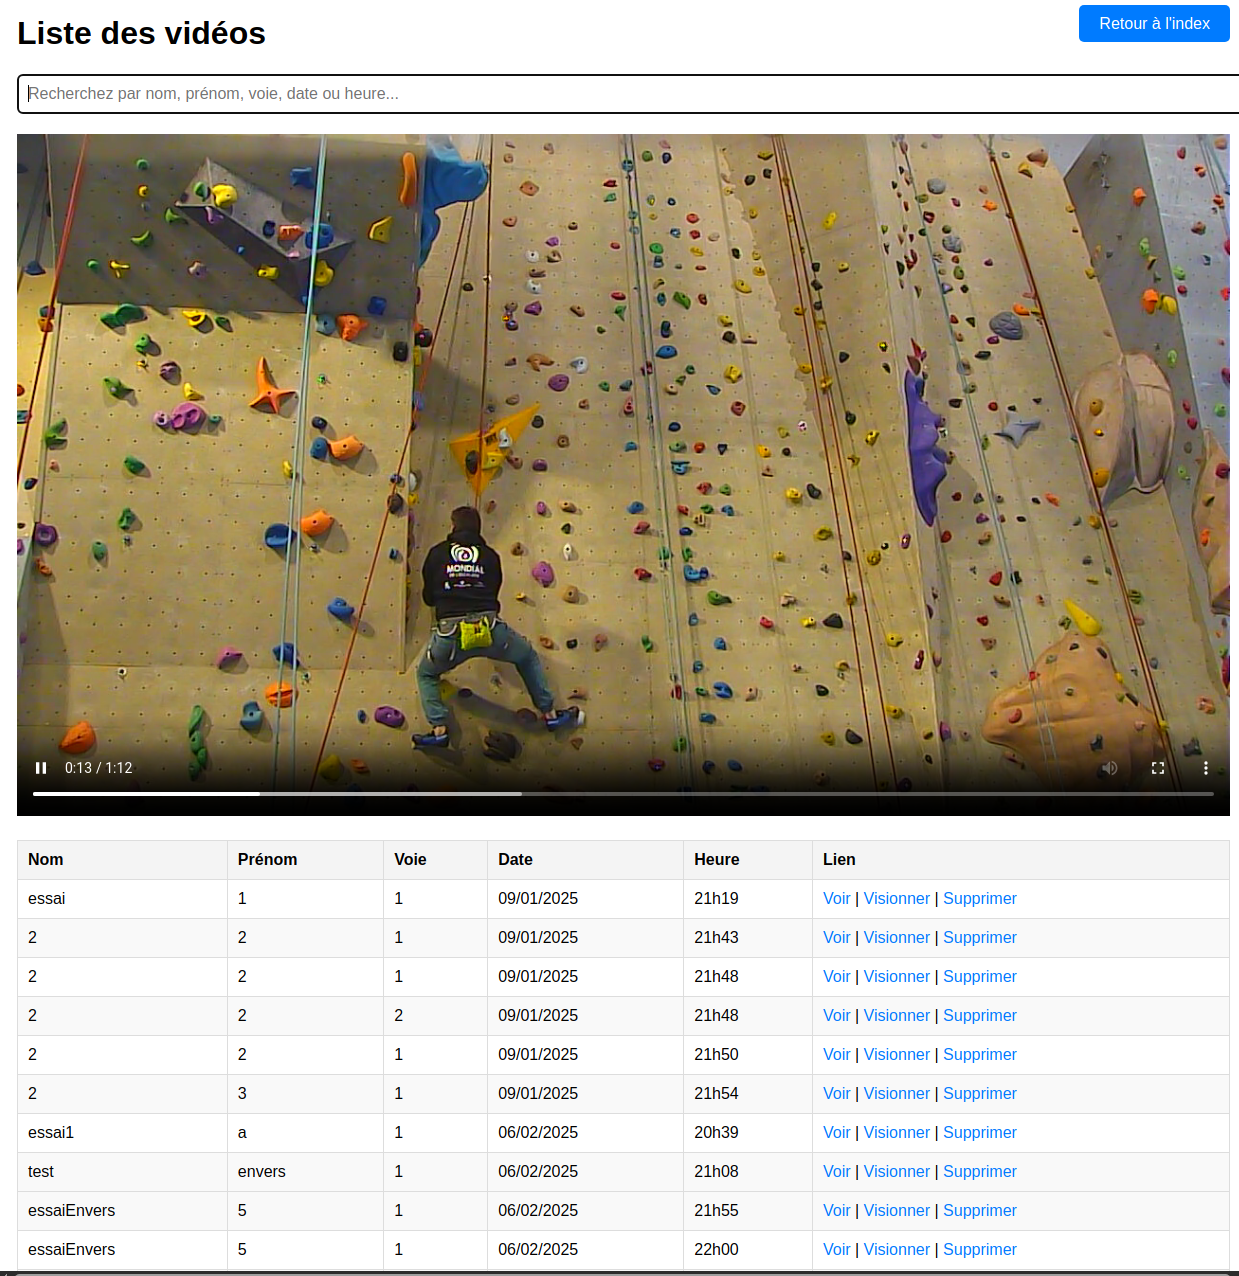
\includegraphics[width=\textwidth]{pageVideo.png}
    \caption{Page web de visualisation des vidéos}
    \label{fig:pageVideo}
  \end{subfigure}
  \caption{Pages web de l'application}
  \label{fig:pagesWeb}
\end{figure}

\subsubsection{Page web index (figure~\ref{fig:pageIndex})}
Au chargement de cette page, une fonction \texttt{javascript} permet de charger les voies disponibles dans la base de données et de les ajouter dans une liste déroulante pour permettre à l'utilisateur de sélectionner la voie qu'il souhaite visualiser. Une seconde fonction \texttt{js} charge les caméras disponibles et les ajoute dans une seconde liste déroulante. Puis le script \texttt{video.cgi} est exécuté pour afficher le flux vidéo de la caméra sélectionnée.

Le processus lit dans la mémoire partagée les images brutes a l'aide d'\texttt{OPENCV} pour récupérer une matrice de pixel, puis le profil colorimétrique de l'image est changé car \texttt{OPENCV} travaille en \textit{BGR (blue green red)} et le \texttt{JPEG} utilise un profil (\textit{RGB (red green blue)}) puis est encodé en \texttt{JPEG} à l'aide de la librairie \texttt{libjpeg}. Enfin, on ajoute les entêtes \texttt{HTTP} pour que le navigateur puisse interpreter l'image et on écrit l'image encodée dans la sortie standard.

Sur la gauche de cette page, on retrouve tout les boutons de contrôle de la caméra (haut, bas, gauche et droite) associé à un curseur pour la précision de l'angle afin de premettre un déplacement plus précis. On retrouve un second curseur pour gérer le zoom de la caméra entre 1x et 18x. La pression de l'un de ses boutons créent une requête \texttt{AJAX} pour exécuter le script \texttt{action.cgi} qui va écrire dans la mémoire partagée l'action à effectuer puis réveiller le programme principal pour qu'il effectue l'action et attendre le feedback du main ou un timeout de 5 secondes avec l'intruction \texttt{SIGALRM} (il récupère le pid du main dans un fichier que ce dernier crée au démarrage). Finalement, il envoie une réponse \texttt{HTTP} pour indiquer que l'action a bien été effectuée.

En dessous de ces curseurs, il y a une liste déroulante pour choisir la voie que l'on souhaite observer. À la selection d'une voie on vient changer de caméra si besoin et la positionner au bon endroit.

En dessous de la video, on retrouve un bouton pour enregistrer une vidéo avec deux champ pour entre le nom et prenom du grimpeur, un exemple de requête \texttt{AJAX} est présenté ci-contre : \texttt{http://localhost/cgi-bin/action.cgi?enrg=on\&nom=Chevalier\&prenom=Romain\&voie=0}. On récupère le nom et la voie afin de produire un nom de fichier unique et pouvoir le récupérer facilement dans la page de visualisation des vidéos.

\paragraph{Paramètres avancés}  En bas de page, on trouve les options pour configurer une nouvelle voie. Il y a une liste déroulante pour choisir la caméra, puis une seconde liste déroulante pour choisir une voie que l'on souhaite supprimer ou afficher sur l'appuie du bouton adéquat. Il y a également un bouton pour sauvegarder une nouvelle position de la caméra dans la base de données en affichant une fenêtre popup pour demander le numéro de voie. 
En addition, on peut également lancer ou stop un enregistrement seul sans suivi du grimpeur et à l'inverse, on peut lancer seulement et stopper la détection du grimpeur sans enregistrement.

\subsubsection{Page web de visualisation des vidéos (figure~\ref{fig:pageVideo})}
Cette page permet de visualiser les vidéos enregistrées, de les télécharger et de les supprimer. Elles sont répertoriées dans un tableau avec le nom du grimpeur, la voie, la date et l'heure de l'enregistrement. On peut, de plus, rechercher une video particulière à l'aide de la barre de recherche en haut de page. Avec les fonction du navigateur, on peut lire, mettre en pause, accélérer, ralentir ou télécharger la vidéo. Enfin, on peut voir la video en haut de page en cliquant sur \texttt{voir}, la visionnier dans un nouvel onglet en cliquant sur \texttt{visionnier} ou la supprimer en cliquant sur \texttt{supprimer}.

















%-----------------------------------------------------------
\section{Tests et résultats}

\section{Perspectives d'amélioration}
\begin{itemize}
  \item Amélioration de l'interface Web, avoir une interface plus intuitive et plus ergonomique.
  \item Reformater le code et tout traduire en anglais
  \item Afficher sur l'écran du Raspberry Pi, un meilleur status de l'execution de l'application.
  \item Utiliser les boutons du Raspberry Pi pour relancer l'application.
  \item Ajouter un système de notification pour les erreurs.
  \item Mieux gérer le stockage des vidéos.
  \item Ajouter un système de détection de chute.
\end{itemize}








%-----------------------------------------------------------
% \clearpage
% \newpage


% \section*{Annexes}
% \addcontentsline{toc}{section}{Annexes}

% \appendix

% \startcontents[sections]
% \printcontents[sections]{l}{1}{\setcounter{tocdepth}{2}}


%     \section{Glossaire}
      




\end{document}